\documentclass[]{book}

%These tell TeX which packages to use.
\usepackage{array,epsfig}
\usepackage{amsmath}
\usepackage{amsfonts}
\usepackage{amssymb}
\usepackage{amsxtra}
\usepackage{amsthm}
\usepackage{mathrsfs}
\usepackage{color}
\usepackage{graphicx}
\usepackage{bm}
\usepackage{tikz}
\usepackage{float}
%\usepackage{widthof}
\usetikzlibrary{arrows}

%Here I define some theorem styles and shortcut commands for symbols I use often
\theoremstyle{definition}
\newtheorem{defn}{Definition}
\newtheorem{thm}{Theorem}
\newtheorem{cor}{Corollary}
\newtheorem*{rmk}{Remark}
\newtheorem{lem}{Lemma}
\newtheorem*{joke}{Joke}
\newtheorem{ex}{Example}
\newtheorem*{soln}{Solution}
\newtheorem{prop}{Proposition}

\newcommand{\lra}{\longrightarrow}
\newcommand{\ra}{\rightarrow}
\newcommand{\surj}{\twoheadrightarrow}
\newcommand{\graph}{\mathrm{graph}}
\newcommand{\bb}[1]{\mathbb{#1}}
\newcommand{\Z}{\bb{Z}}
\newcommand{\Q}{\bb{Q}}
\newcommand{\R}{\bb{R}}
\newcommand{\C}{\bb{C}}
\newcommand{\N}{\bb{N}}
\newcommand{\M}{\mathbf{M}}
\newcommand{\m}{\mathbf{m}}
\newcommand{\MM}{\mathscr{M}}
\newcommand{\HH}{\mathscr{H}}
\newcommand{\Om}{\Omega}
\newcommand{\Ho}{\in\HH(\Om)}
\newcommand{\bd}{\partial}
\newcommand{\del}{\partial}
\newcommand{\bardel}{\overline\partial}
\newcommand{\textdf}[1]{\textbf{\textsf{#1}}\index{#1}}
\newcommand{\img}{\mathrm{img}}
\newcommand{\ip}[2]{\left\langle{#1},{#2}\right\rangle}
\newcommand{\inter}[1]{\mathrm{int}{#1}}
\newcommand{\exter}[1]{\mathrm{ext}{#1}}
\newcommand{\cl}[1]{\mathrm{cl}{#1}}
\newcommand{\ds}{\displaystyle}
\newcommand{\vol}{\mathrm{vol}}
\newcommand{\cnt}{\mathrm{ct}}
\newcommand{\osc}{\mathrm{osc}}
\newcommand{\LL}{\mathbf{L}}
\newcommand{\x}{\bm{x}}
\newcommand{\UU}{\mathbf{U}}
\newcommand{\support}{\mathrm{support}}
\newcommand{\AND}{\;\wedge\;}
\newcommand{\OR}{\;\vee\;}
\newcommand{\Oset}{\varnothing}
\newcommand{\st}{\ni}
\newcommand{\wh}{\widehat}

%Pagination stuff.
\setlength{\topmargin}{-.3 in}
\setlength{\oddsidemargin}{0in}
\setlength{\evensidemargin}{0in}
\setlength{\textheight}{9.in}
\setlength{\textwidth}{6.5in}
\pagestyle{empty}



\begin{document}

\begin{center}
{\Large Draft}\\
\textbf{Alireza Abrehforoush}\\ %You should put your name here
Date: 8-10-2022 %You should write the date here.
\end{center}
\vspace{0.2 cm}
%%%%%%%%%%%%%%%%%%%%%%%%%%%%%%%%%%%%%%%%%%%
\section{Configurations with more than two red arcs of length one (asynchronous)}
\begin{figure}[H]
    \centering
    \includegraphics[width=0.4\textwidth]{figures/pic2.jpg}
    \caption{configuration with $\left(c_{1}, c_{2}, c_{3}, c_{4}, c_{5}, c_{6}\right) = \left(5, 4, 0, 3, 0, 0\right)$}
    \label{fig:mesh2}
\end{figure}
Corresponding to all configurations with $i$ red arcs of length one (for simplicity from now on we call it red arcs), we consider a \emph{system} $i^\prime$ in which our random walker is wandering and leaves it after a while. as in asynchronous dynamics the number of red arcs is descending and at each time at most two red arcs can disappear (by activation of the agent adjacent to two red arcs), these systems can be modeled through below directed path graphs regarding the parity of number of red arcs of length one at the beginning ($m$):

%graph
\begin{figure}[H]
    \centering
    \begin{tikzpicture}
    \tikzset{vertex/.style = {shape=circle,draw,minimum size=3em}}
    \tikzset{edge/.style = {->,> = latex'}}
    % vertices
    \node[vertex] (a) at  (-6,0) {$0^\prime$};
    \node[vertex] (b) at  (-2,0) {$2^\prime$};
    \node[vertex] (c) at  (2,0) {$4^\prime$};
    \node[vertex] (d) at  (6,0) {$m^\prime$};
    %edges
    \path[->] (b) edge
    node[above]{} (a);
    \path[->] (c) edge
    node[above]{} (b);
    
    \path (c) to node {\dots} (d);
    \end{tikzpicture}
    \caption{systems starting with at most even number of red arcs of length one ($m$)}
\end{figure}
%graph
%graph
\begin{figure}[H]
    \centering
    \begin{tikzpicture}
    \tikzset{vertex/.style = {shape=circle,draw,minimum size=3em}}
    \tikzset{edge/.style = {->,> = latex'}}
    % vertices
    \node[vertex] (a) at  (-6,0) {$1^\prime$};
    \node[vertex] (b) at  (-2,0) {$3^\prime$};
    \node[vertex] (c) at  (2,0) {$5^\prime$};
    \node[vertex] (d) at  (6,0) {$m^\prime$};
    %edges
    \path[->] (b) edge
    node[above]{} (a);
    \path[->] (c) edge
    node[above]{} (b);
    
    \path (c) to node {\dots} (d);
    \end{tikzpicture}
    \caption{systems starting with at most odd number of red arcs of length one ($m$)}
\end{figure}
%graph

We denote the upper bound of stay time of our random walker on expectation in system $i$ by $T_{i}$. so the expected time to reach equilibrium starting from any arbitrary configuration ($T$) is the expected time of reaching from system $m^\prime$ to system $0^\prime$:

\begin{equation}
    T = \sum_{i = 0}^{m} T_i
\end{equation}

For computing $T$ we have two following approaches:
\subsection{Using  part 1}

$X$ and $Y$ (red arcs in below figure) are the first two red arcs that disappear in this configuration (Obviously $X$ and $Y$ are two adjacent red arcs). Thus we ignore other unstable arcs (shown with pink).

\begin{figure}[ht]
    \centering
    \includegraphics[width=0.4\textwidth]{figures/m.arcs.jpg}
    \caption{}
    \label{fig:mesh3}
\end{figure}


We can model problem through following Markov chain. Assuming $X$ and $Y$ are the first two red arcs that disappear, state $i$ corresponds to the configuration in which $i$ black arcs exist between $X$ and $Y$. So the probability of reaching to system $(m-2)^\prime$ through states $1$ to $n-m$ in one step is zero.

%graph
\begin{figure}[H]
    \centering
    \begin{tikzpicture}
    \tikzset{vertex/.style = {shape=circle,draw,minimum size=3em}}
    \tikzset{edge/.style = {->,> = latex'}}
    % vertices
    \node[vertex] (b) at  (-3,3) {$n-m+1$};
    \node[vertex] (b2) at  (0,3) {$n-m+2$};
    \node[vertex] (b3) at  (5,3) {$n-1$};
    
    \node[vertex] (a) at  (-4,0) {$0$};
    \node[vertex] (c) at  (6,0) {$n-m$};
    \node[vertex] (d) at  (1,-3) {$(m-2)^\prime$};
    \node[vertex] (a1) at (-2,0) {$1$};
    \node[vertex] (a2) at (0,0) {$2$};
    %edges
    \draw[->] (a) edge  [loop above] node {$1-3p$} ();
    \draw[->] (b) edge  [loop above] node {$1$} ();
    \draw[->] (b2) edge  [loop above] node {$1$} ();
    \draw[->] (b3) edge  [loop above] node {$1$} ();
    \draw[->] (c) edge  [loop above] node {$1-2p$} ();
    \draw[->] (a1) edge  [loop above] node {$1-4p$} ();
    \draw[->] (a2) edge  [loop above] node {$1-4p$} ();
    
    \path[->] (a) edge[bend right]      node[above]{$p$} (d);
    
    \path[->] (a) edge[bend left]     node[above]                      {2p} (a1);
    \path[->] (a1) edge[bend left]     node[above]                      {2p} (a);
    
    \path[->] (a1) edge[bend left]     node[above]                      {2p} (a2);
    \path[->] (a2) edge[bend left]     node[above]                      {2p} (a1);

    %
    \path (b2) to node {\dots} (b3);
    %
    
    \path (a2) to node {\dots} (c);
    \node [shape=circle,minimum size=1.5em] (a3) at (2,0) {};
    \path[->] (a2) edge[bend left]     node[above]                      {2p} (a3);
    \path[->] (a3) edge[bend left]     node[above]                      {2p} (a2);
    
    \node [shape=circle,minimum size=1.5em] (c1) at (4,0) {};
    \path[->] (c) edge[bend left]     node[above]                      {2p} (c1);
    \path[->] (c1) edge[bend left]     node[above]                      {2p} (c);
    \end{tikzpicture}
    \caption{system with $m$ red arcs}
\end{figure}
%graph

We consider states $0, 1, \hdots, n$ corresponding to the configurations with $c = i \in \{0, 1, . . . , n\}$. Let $t_c$ denote the expected transition time from system $m^\prime$ to $(m-2)^\prime$, starting from state $c$. The changes in $c$ are governed by the following recursive equation:
\begin{equation}
    t_c 
    = 2p t_{c-1}  + 2p t_{c+1} + (1 - 4p)t_{c} + 1\\
    = \frac{1}{2}t_{c-1} + \frac{1}{2}t_{c+1} + \frac{1}{4p}, \qquad c = 1,\ldots,n-m-1,
\end{equation}
with following initial conditions:
\begin{equation}
\begin{split}
    &t_0 = p\times 0 + 2pt_1 + (1-3p)t_0  + 1 = \frac{2}{3}t_1 + \frac{1}{3p} \\
    &t_{n-m} = 2pt_{n-m-1} + \left( 1-2p \right)t_{n-m} = t_{n-m-1} + \frac{1}{2p}
\end{split}
\end{equation}
From (2) and (3) we can infer
\begin{multline*}
    \\
    t_1 = \frac{1}{2}t_0 + \frac{1}{2}t_2 + \frac{1}{4p}\\
    t_2 = \frac{1}{2}t_1 + \frac{1}{2}t_3 + \frac{1}{4p}\\
    t_3 = \frac{1}{2}t_2 + \frac{1}{2}t_4 + \frac{1}{4p}\\
    \vdots\\
    t_{n-m-1} = \frac{1}{2}t_{n-m-2} + \frac{1}{2}t_{n-m} + \frac{1}{4p}\\
    \sum_{i=1}^{n-m-1} t_i = \frac{1}{2}\left[ \sum_{i=0}^{n-m-2} t_i + \sum_{i=2}^{n-m} t_i \right] + \frac{n-m-1}{4p} \Rightarrow t_1 + t_{n-m-1} = \frac{1}{2}\left(t_0 + t_1 + t_{n-m-1} + t_{n-m}\right) + \frac{n-m-1}{4p}\\
    \Rightarrow t_1 + t_{n-m-1} = t_0 + t_{n-m} + \frac{n-m-1}{2p}
\end{multline*}

Using (3) we can infer

\begin{center}
\begin{equation}
    t_1 = \frac{2}{3}t_1 + \frac{1}{3p} + \frac{1}{2p} + \frac{n-m-1}{2p} \Rightarrow t_1 = \frac{3n-3m+2}{2p}
\end{equation}
\begin{equation}
    t_0 = \frac{2}{3}t_1 + \frac{1}{3p} = \frac{n-m+1}{p}
\end{equation}
\end{center}

We now have a non-homogeneous linear recurrence relation with (2) as relation and (4) and (5) as initial conditions. The solution ($t_c$)
of a non-homogeneous recurrence relation has two parts.
First part is the solution ($t^{(h)}_{c}$)
of the associated homogeneous recurrence relation and the second part is the particular solution ($t^{(p)}_{c}$).
$$
        t_c = t^{(h)}_{c} + t^{(p)}_{c}
$$
First we rewrite (2) in standard form.
\begin{equation}
    t_{c+1} = 2t_c - t_{c-1} - \frac{1}{2p}
\end{equation}
The characteristic polynomial corresponding to the homogeneous part is as follows:
$$
r^2 - 2r + 1 = 0 \Rightarrow r = 1
$$
Thus the general solution is of the form
$$
t_c = \alpha_{1}c 1^c + \alpha_{2} 1^c
$$
Armed with that knowledge, and since the non-homogeneous part is also a polynomial (in this case of degree zero) which is itself a degenerate case of being of the form $1^c$ as well, we multiply by $c$ enough times to make it distinct from the other already known parts. I.e. we expect the non-homogeneous part to be of the form $\beta c^2$. Plugging this into the recurrence, we have:
$$
\beta (c+1)^2 = 2\beta c^2 - \beta (c-1)^2 - \frac{1}{2p} \Rightarrow \beta = -\frac{1}{4p}
$$
So, we expect
$$
t_c = \alpha_1 c + \alpha_2 - \beta c^2 = \alpha_1 c + \alpha_2 -\frac{1}{4p}c^2
$$
using initial conditions we have:
$$
t_0 = \alpha_1 \times 0 + \alpha_2 - \frac{1}{4p}\times 0 = \frac{n-m+1}{p} \\
\Rightarrow \alpha_2 = \frac{n-m+1}{p}
$$
and
$$
t_1 = \alpha_1 + \frac{n-m+1}{p} -\frac{1}{4p} = \frac{3n-3m+2}{2p} \Rightarrow \alpha_1 = \frac{2n-2m+1}{4p}
$$
Thus, the final closed form is:
\begin{equation}
    t_c = \frac{(c+2)(2n-2m) - c^2 + c + 4}{4p}\\
    \qedsymbol
\end{equation}
From (1) and the fact that the number of red arcs can not be more than $n$, the upper bound for expected equilibrium time is $O(n^3)$.

\newpage
\subsection{Using recurrence relation}
Consider a configuration with $m$ red arcs which the distance between each two of them is an integer from the set $\left\{ 0,1,2,\hdots,n-1 \right\}$. We can denote this configuration by $\left( c_{1}, c_{2}, \hdots, c_{m} \right)$ (and any circular shift of the distances). Let $t_{c_{1},c_{2},\hdots,c_{m}}$ denote the expected equilibrium time, starting from state $\left( c_{1}, c_{2}, \hdots, c_{m} \right)$. The changes in $\left( c_{1}, c_{2}, \hdots, c_{m} \right)$ in any arbitrary configuration are governed by the following recursive
equation:
\begin{equation}
\begin{split}
    \forall i: c_i \neq 0 \qquad
    t_{c_1, c_2, \hdots, c_m} &= \sum_{i = 1}^{m} pt_{c_1, \hdots, c_{i}-1, c_{i+1}+1, \hdots, c_m} + pt_{c_1, \hdots, c_{i-1}+1, c_{i}-1, \hdots, c_m} \\
    &+ \left(1 - 2mp\right)\left( t_{c_{1}, c_{2}, \hdots, c_{m}} \right) \\
    &+ 1
\end{split}
\end{equation}
and following initial conditions (every configuration with at least one black arc of length 0):
\begin{equation}
\begin{split}
    \chi = \left\{ i:c_i = 0 \right\} \qquad t_{c_1, c_2, \hdots, c_m} &= \sum_{i \notin \chi} pt_{c_1, \hdots, c_{i}-1, c_{i+1}+1, \hdots, c_m} + pt_{c_1, \hdots, c_{i-1}+1, c_{i}-1, \hdots, c_m} \\
    &+ \sum_{i \in \chi} pt_{c_1, \hdots, c_{i-2}, c_{i-1} + 2 + c_{i+1}, c_{i+2}, \hdots, c_m} \\
    &+ \left( 1 - |\chi| - 2|\chi^\prime| \right)pt_{c_1, c_2, \hdots, c_m} \\
    &+ 1
\end{split}
\end{equation}






\end{document}